\documentclass[journal]{vgtc}                % final (journal style)
%\documentclass[review,journal]{vgtc}         % review (journal style)
%\documentclass[widereview]{vgtc}             % wide-spaced review
%\documentclass[preprint,journal]{vgtc}       % preprint (journal style)

%% Uncomment one of the lines above depending on where your paper is
%% in the conference process. ``review'' and ``widereview'' are for review
%% submission, ``preprint'' is for pre-publication, and the final version
%% doesn't use a specific qualifier.

%% These few lines make a distinction between latex and pdflatex calls and they
%% bring in essential packages for graphics and font handling.
%% Note that due to the \DeclareGraphicsExtensions{} call it is no longer necessary
%% to provide the the path and extension of a graphics file:
%% 
\includegraphics{diamondrule} is completely sufficient.
%%
\ifpdf%                                % if we use pdflatex
  \pdfoutput=1\relax                   % create PDFs from pdfLaTeX
  \pdfcompresslevel=9                  % PDF Compression
  \pdfoptionpdfminorversion=7          % create PDF 1.7
  \ExecuteOptions{pdftex}
  \usepackage{graphicx}                % allow us to embed graphics files
  \DeclareGraphicsExtensions{.pdf,.png,.jpg,.jpeg} % for pdflatex we expect .pdf, .png, or .jpg files
\else%                                 % else we use pure latex
  \ExecuteOptions{dvips}
  \usepackage{minted}
  \usepackage{graphicx}                % allow us to embed graphics files
  \DeclareGraphicsExtensions{.eps}     % for pure latex we expect eps files
\fi%

%% it is recomended to use ``\autoref{sec:bla}'' instead of ``Fig.~\ref{sec:bla}''
\graphicspath{{figures/}{pictures/}{images/}{./}} % where to search for the images

\usepackage{microtype}                 % use micro-typography (slightly more compact, better to read)
\PassOptionsToPackage{warn}{textcomp}  % to address font issues with \textrightarrow
\usepackage{textcomp}                  % use better special symbols
\usepackage{mathptmx}                  % use matching math font
\usepackage{times}                     % we use Times as the main font
\renewcommand*\ttdefault{txtt}         % a nicer typewriter font
\usepackage{cite}
\usepackage{caption}
\usepackage{array}

%% If you are submitting a paper to a conference for review with a double
%% blind reviewing process, please replace the value ``0'' below with your
%% OnlineID. Otherwise, you may safely leave it at ``0''.
\onlineid{0}

%% declare the category of your paper, only shown in review mode
\vgtccategory{Research}

%% Paper title.
\title{Visualizing the Los Angeles Metro Bikeshare System}

%% This is how authors are specified in the journal style
%% indicate IEEE Member or Student Member in form indicated below
\author{Prathyusha Butti, Pratik Bhandari and Ripan Chowdhury}
\authorfooter{
%% insert punctuation at end of each item
\item
 \author{Prathyusha Butti, Pratik Bhandari and Ripan Chowdhury}
 are graduate students at the University of Arizona.
 
E-mail:pbutti@email.arizona.edu. 
E-mail:pratikbhandari@email.arizona.edu.
E-mail:rchowdhury1@email.arizona.edu.
}

%other entries to be set up for journal
%\shortauthortitle{Firstauthor \MakeLowercase{\textit{et al.}}: Paper Title}

%% Abstract section.
\abstract{
Bike sharing systems are gaining immense popularity as an alternative or complementary mode of urban transport. Bike sharing can provide an alternative to traditional modes of transport or, more likely a complementary service for solving the "last mile problem" of getting from a public transportation stop to the final destination. Furthermore, bike sharing systems may help mitigate automobile congestion and reduce pollution, although relatively little research has been done to asses their actual impact in these areas. Visualizing and analyzing the current operations can assist in getting a better grasp on the performance of the system. In this paper, a data visualization approach is used to identify important factors related to the bike-sharing system. We analyzed the bike-sharing system such that we were able to group the bike renting trends, locate the busiest stations in the locality and number of monthly or flex passes taken by the customers for different time granularity. We have mined the Metro Bike Share, Los Angeles data and discussed the findings of this data set. Using this publicly available data, we conducted some experiments combining data filters and visualizations, potentially analyzing the sustainability of the bike sharing system.
For this milestone, we have expanded on our progress from the fourth milestone. One of the major tasks was to conduct evaluation by showing our visualization to other people who aren't from visualization domain and get their feedback and the other part was to present our visualization in the class and get the feedback from fellow students. The reports and analysis which will be further discussed in the evaluation section. 

} % end of abstract

%% Keywords that describe your work. Will show as 'Index Terms' in journal
%% please capitalize first letter and insert punctuation after last keyword
\keywords{Bike-Share, Visualization, Clustering, Data Mining.}

%% ACM Computing Classification System (CCS). 
%% See <http://www.acm.org/class/1998/> for details.
%% The ``\CCScat'' command takes four arguments.

%\CCScatlist{ % not used in journal version
% \CCScat{K.6.1}{Management of Computing and Information Systems}%
%{Project and People Management}{Life Cycle};
% \CCScat{K.7.m}{The Computing Profession}{Miscellaneous}{Ethics}
%}

%% Uncomment below to include a teaser figure.
%   \teaser{
%   \centering
%   \includegraphics[width=16cm]{CypressView}
%   \caption{In the Clouds: Vancouver from Cypress Mountain.}
%  }

%% Uncomment below to disable the manuscript note
\renewcommand{\manuscriptnotetxt}{}

%% Copyright space is enabled by default as required by guidelines.
%% It is disabled by the 'review' option or via the following command:
% \nocopyrightspace

\vgtcinsertpkg

%%%%%%%%%%%%%%%%%%%%%%%%%%%%%%%%%%%%%%%%%%%%%%%%%%%%%%%%%%%%%%%%
%%%%%%%%%%%%%%%%%%%%%% START OF THE PAPER %%%%%%%%%%%%%%%%%%%%%%
%%%%%%%%%%%%%%%%%%%%%%%%%%%%%%%%%%%%%%%%%%%%%%%%%%%%%%%%%%%%%%%%%

\begin{document}

%% The ``\maketitle'' command must be the first command after the
%% ``\begin{document}'' command. It prepares and prints the title block.

%% the only exception to this rule is the \firstsection command
\firstsection{Overview} % or "Motivation"

\maketitle

\label{sec:overview}
Bike share schemes are an increasingly prevalent mode of intra-city transportation. The concept of bike sharing systems was introduced in 1965 Amsterdam. A bike sharing program is a system of supplying bikes for hire for point-to-point transportation. This program enables convenient active transportation as people have an option to ride between two stations in a defined geographical area. Since the introduction of bike-sharing systems, much research has been dedicated to different aspects of these systems. The benefits of bikes in urban areas, where travel distance is short, and the parking prices are high, has caused the demand for bike-sharing systems to increase. Bike share systems may help mitigate automobile congestion and reduce pollution, although relatively little research has been done to assess their actual impact in these areas. Benefits to users include potentially reduced commute times by perhaps as much as 10\% \cite{Sakari:2013:Data} and a healthier lifestyle to lead. 
 
Besides visualizing bike sharing systems as a new means of public transportation, such community shared programs offer a new way to look into the dynamics of movements inside a city, and more generally into its activity. In a sense, it provides digital footprints that reveal the activity of people in the city over time and space and makes possible their analysis. Different issues motivate the study of such a system. Some questions are about the usage patterns of this kind of transport, with reference to social or economic studies of transportation, while others are about the system itself: does the service work correctly? Can it be optimized? Can one regulate the availability of bikes? Some of the studies related to this system are descriptive and mine the data to get a better understanding of the operations. 

Data Visualization and analysis of the current operations can assist in getting a better grasp on the performance of the system. Data visualization, which is defined as the effort of placing data in a visual context, can assist in better understanding the problem. When we have many data points, the visualization of the data becomes challenging. The purpose of this study is to analyze the bike-sharing system by applying filters like renting trends. We have mined the Metro Bike Share, Los Angeles data and discussed the findings of this data set. We have examined the bike-share system during different quarters of the year, therefore potentially analyzing the sustainability of the bike sharing system. This study also helped us in gaining a better understanding of the urban mobility of Los Angeles residents. In terms of visualizations, our project does not develop a novel visualization but uses prevalent methods of visualizing data to try and find trends of a certain behavior from this dataset. We have analyzed various types of visualizations and brought together several ideas to form an interactive and easy-to-use interface that helps users navigate through the bike-sharing data in a more ordered and systematic way. Our choice of visualization holds ground with the design practices that make an effective visualization and also takes into consideration some design techniques that further enhance the user experience.

The following progress has been made for this milestone:
\begin{itemize}
  \item \textbf{Presentation}: We have a presented our visualization on November 21st, 2018 to the class and recieved their feedback.  
  \item \textbf{Evaluation}: We have designed our evaluation and received results from different users and have analyzed them in the evaluation section.

\end{itemize}
 

\input{visualization_progress}
%%\section{Task and Data Abstraction} 
\label{sec:task_and_data_abstraction}

We initially obtained our data from a popular online data source, Kaggle. The dataset was named \textit{Los Angeles Metro Bike Share Trip Data}. Even though this dataset had enough depth to reason about various trends and patterns, it was less in number which made us look for other sources of similar data. We then found a substantial amount of data in Bike Share Metro, which seemed to fulfill our requirements for this project. This data, like the one before, is from Los Angeles and contains the shared bike ride information for 2.5 years, 2016 Q3 to 2018 Q2. 
The dataset is in Table form and the table has all total 14 attributes. They are:
\begin{itemize}
    \item trip\_id - Unique ID for a particular trip
    \item duration - Duration of the trip in minutes
    \item start\_time - Start time of the trip
    \item end\_time - End time of the trip
    \item start\_lon - Starting position longitude
    \item start\_lat - Starting position latitude
    \item start\_station - The station ID where the trip originated
    \item end\_station -  The station ID where the trip terminated
    \item end\_lat - Destination latitude
    \item end\_lon - Destination longitude
    \item bike\_id - Id for each bike
    \item plan\_duration - Duration of the customer's plan
    \item passholder\_type - The name of the pass holder's plan
    \item trip\_route\_category\ -  "Round Trip" for trips starting and ending at the same station or "One Way" for all other trips
\end{itemize}
Moreover, there are four spatial attributes in the datasets, namely, start\_lon, start\_lat, end\_lon and end\_lat. We will be using the trip\_id as the key for each item.

\subsection{Task Abstraction}
\label{sec:task}
All the data about bike share venture we could gather focus mainly on the number of customers, duration of their trips and the locations from which the bikes are rented. So, our aim is to analyze which places see the maximum number of business each day, moreover how the business is growing over time. The goals identified by us are the following:

\begin{itemize}
    \item G1: Get a mental picture of business according to location:
    It will be very helpful in analyzing the viability of the bike share system if we could get a mental picture, around which geographic locations most of the business tend to gather. If there was a visible comparison between different locations, it would be so much easier to comprehend where the focus of the business should be, moreover if we can find some connection between high volume of the rentals at those locations, the same model could also be implemented in other locations with similar potential. The idea of business can be explained by the number of drop-offs and hires from a specific station. Typically, a station having a high number of hires has more business. We will also check for stations where both drop-offs and hires are high. These can be considered as locations with high business. By mapping the drop-off i.e. (end\_longitude, end\_latitude) and hire i.e. (start\_longitude, start\_latitude) over the geographic map, we can get a good sense of our task.

    \item G2:  How the customers’ preferences are changing over time
    There are three kinds of passes available for the customers, namely walkup (daily), monthly and flex (annual). They provide one day, one month and year-round rental service respectively. If we could find the trends in the change in the number of passes over different time granularity, we could get a clear picture of the preferences of the customers. The time granularity can be either months or quarters or years.
    
    \item G3: How the volume of the rentals changes over time:
    If we can visualize how the number of customers changes over time, it will also provide us with clarifications about which time of the year people tend to chose this form of transport over others. That would be beneficial to understand what compels them to eschew bikes over the other time of the years and what steps could be taken to alleviate their discomfort.
 
\end{itemize}

To identify the smaller task in support of the goals, we can take the following steps.

\begin{itemize}
    \item T1: Comparing the aggregate rentals from different regions:
    We can try to visualize the number of rentals from different geographic locations from the start\_lon and start\_lat attributes from the dataset. The total number of customers from the specific bike stations from different locations can be helpful in getting insights about the viability and the fruitfulness of this venture in different locations.

    \item T2: Comparing rentals at different time of the years:
    We have the data on the number of rentals according to the different quarters of the years from 2016 to 2018. So if the user wants to zoom into the visualization using a context + focus design approach, it would also be apparent how the number of rentals is changing along the different times of the year.

    \item T3: Comparing the passes throughout the years:
    We can make the comparisons between the different kinds of passes over different quarters/months of different years. We can show this way how many passes from the three categories are getting sold each at each time level. Moreover, it can give us some insights about which pass generates the most amount of revenue and which one is the best option for holding on to customer loyalty and thus garnering and maintaining the reputation for the company.
\end{itemize}

Summary: All the visualizations necessary here tend to focus on the comparisons, discovery, and identification to some extent. We can use these task abstractions and objectives as further guides to our design selection process.

%%\section{Preliminary Designs} 
\label{sec:preliminary_designs}

In the course of research and discussions about possible visualization to implement for our project, we came up with a number of suitable visualizations that seemed suitable to use in our project. Below is the list and description of each visualization along with reasoning to support our choice of this visualization.

\subsection{Pick-Up vs Drop-Off}
\label{sec:viz1}

The first design we thought of was a geographical map which plots the arrival and departure areas of the share-bikes and maps this data according to their frequency. So, for this visualization, a geometrical plot was being used. Here the marks were the share-bikes (either arriving or departing) and the attribute was the frequency of arrival or departure. We planned on using circles to denote the arrival or departure at the bike station. This way, the mark of the visualization could be considered as a circle. Since we will be mapping both the arriving and departing bikes, it would be confusing to have circles of both types of data of the same color. Hence, we decided to denote departing and arriving bikes by red and blue color respectively. Similarly, the frequency of arrival/departure would be encoded by the area of the circle (encoding rule). The channels here are the geographical (x and y) positions, color and area. 

This choice of visualization was directly influenced by similar work \cite{UrbanDataCyclist} done by Daniel Peterson, where they mapped hires and drop-offs on a location with circles and encoded the frequency with the area of the circle. The following design is from the above-mentioned study itself.
\begin{figure}[h]
	\centering % avoid the use of \begin{center}...\end{center} and use \centering instead (more compact)
	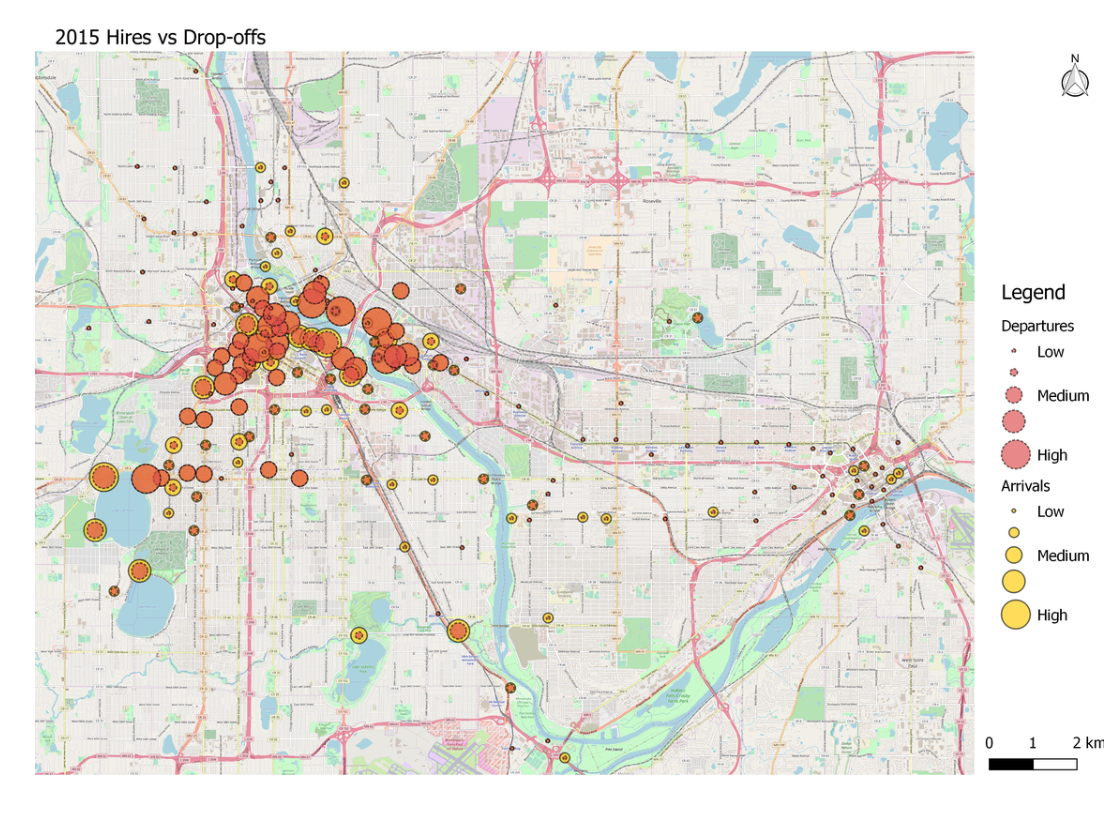
\includegraphics[scale=0.36]{figs/first_viz.PNG}
	\caption{\footnotesize{Mapping hires and drop-offs by circle area. \cite{UrbanDataCyclist}}}
	\label{fig:First viz Chart}
	\captionsetup{justification=centering,margin=1cm}
	\vspace{-10pt}
\end{figure}
\newline
This choice of visualization adheres with much of the design principles studied in our class. It follows the principle of effectiveness as the data is easily separable. By using a single channel (color) to distinguish between hires and drop-offs of bikes is more effective than using 2 channels for it. Also, we were planning to make this an unconstrained navigation which allows more freedom to the user to navigate. On the topic of task abstraction, this visualization is suitable to locate areas of high business activity. The area of circle directly correlates with the idea of high business volume.

In addition to that, the choice of color itself (red and blue) are easy to distinguish and hence are easily separable. These colors do not generally mesh with the mostly green and gray geographical background as well. This choice of visualization helps in the comparison between the hire data and drop-off data. In addition to that, it also helps in comparing the same kind of data (hires or drop-offs) with each other based on different locations. One drawback of this visualization is that the area of the circle does not give a quantitative value of the frequency of hires/drop-offs from the visualization itself. 

\subsection{PassType Mapping with Time}
\label{sec:viz2}

One of the things we were interested in the bike-sharing data was analyzing the bike pass types and their trend. For the bike-sharing service we chose, there are 3 kinds of passes -- daily, monthly and annual. Analysis of these bike-passes with a time of different granularity was not found in other visualization projects and research papers. This encouraged us to take on this concept to find some pattern or trend with this data. 

For this visualization, we planned on using line graph how the number of passes of each kind being bought for different levels of time granularity. The granularity levels could be a month, quarter or year. This option could be selected by the user from a drop-down box to the right of the line graph. Within the line graph, three lines represented the three types of passes. The choice of colors was red, blue and green. This triplet of colors form the basis of the RGB-colorspace which goes to prove that they are distinct from one another when used together. 

The X-axis would be the time axis and the Y-axis would be the magnitude axis. Here, the task abstraction shifts more towards the discovering and analyzing side. Our aim was to find some sort of trend moving forward with time. We expected to see an increase in monthly passes and a slight increase in annual passes. This would indicate that the bike-sharing service is getting popular with time. A more visible change could be perceived if the time was on a level of the year. On the other hand, the daily passes data would give a whole different perspective on how people use these services. By generalizing weather over months i.e. December-March for Winter, we could check if fewer people use the service during winters and more during spring/summer. 

In addition to the task abstraction, this visualization followed the principles of effectiveness and expressiveness as well. It is clearly distinguishable and it encodes only the required values. Being line graph, the level of accuracy is pretty good. Here, we have applied the principle of superimposing by overlaying the line graph of all 3 pass types into a single chart. Our assumption was that this number of overlay won't harm the distinguishability of the lines. Allowing the user to change the time granularity also helps in bringing user interactiveness into the picture. A rough sketch of what the visualization would probably look like is given below:
\begin{figure}[h]
	\centering % avoid the use of \begin{center}...\end{center} and use \centering instead (more compact)
	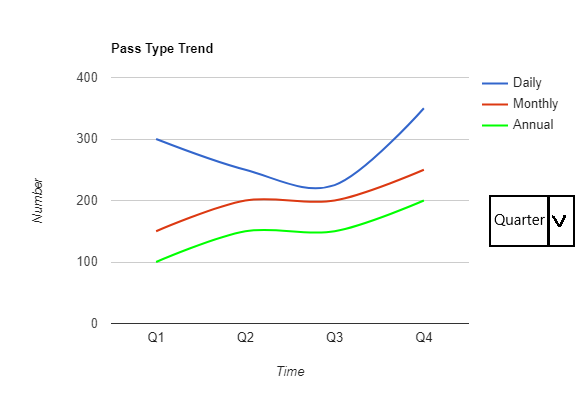
\includegraphics[scale=0.45]{figs/bar-graph.png}
	\caption{\footnotesize{Mapping of pass type with time granularity}}
	\label{fig:Second viz Chart}
	\captionsetup{justification=centering,margin=1cm}
	\vspace{-10pt}
\end{figure}
\newline

\subsection{Crossfilter Based Geographic Mapping}
\label{sec:viz3}

For the final design, we thought of implementing a crossfilter enabled geographic mapping of data. Basically, we will be expanding on the first visualization choice in this list. The difference here is that in the first visualization, the time range has been fixed beforehand. So there is no user interactivity in that visualization. On the other hand, this visualization adds a dynamic element to the previous static visualization. Here, we will have a geographic map just as in the first choice. We plan on mapping the drop-offs and hires just like in the first visualization. The data represented in the geographic plane can be controlled by a slider that can move through a time histogram. The time histogram will map the average duration of a trip for that period of time. So in this way, we can get even more insight into the trend in bike-sharing services.

By averaging the trip duration over a month, and creating a histogram with time as the X-axis and time in minutes as the Y-axis we can look for trends in the trip duration with respect to time. This can give us insights over the fact if people tend to use the bike-share for a longer duration during the summer over the winter. The trip duration might end up being completely independent to the month of the year as well, which is another observation in its own. 

Here, the geographic data can be used to check whether the station placement is optimum or not. If there are more high-frequency drop-offs and hires in a specific location, increasing the bike count in those areas might increase service even more. The histogram is in itself a good visualization and follows the basic design principles pretty well along with providing a high level of accuracy to data and a good form of comparison between data. Furthermore, filtering the geographic data with time gives us an idea of how frequently the bike-sharing service gets used with respect to time. This helps us in our task abstraction defined in the previous section. In addition to all this, having the means to interact and change data in real time is highly user-friendly and will be user-accepted as well. Below is a general mock-up of how the visualization might look like.
\begin{figure}[h]
	\centering % avoid the use of \begin{center}...\end{center} and use \centering instead (more compact)
	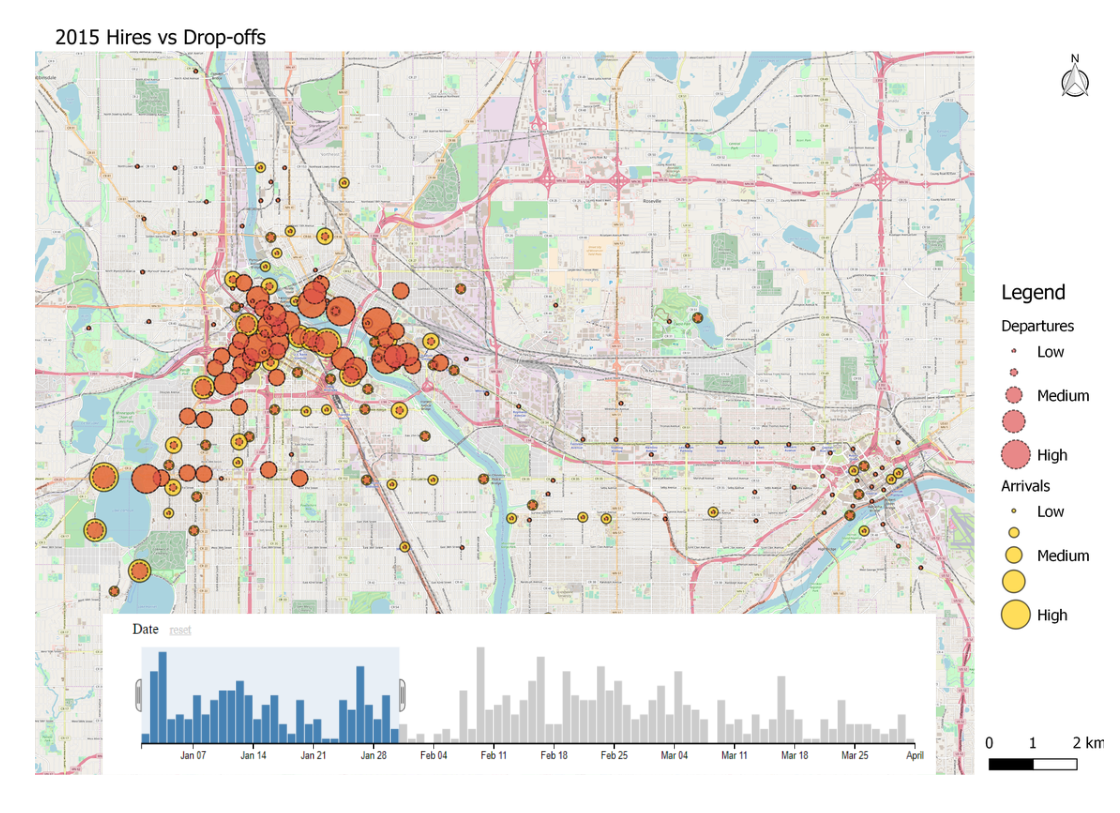
\includegraphics[scale=0.35]{figs/third_viz.PNG}
	\caption{\footnotesize{Crossfilter Enabled Mapping}}
	\label{fig:Third viz Chart}
	\captionsetup{justification=centering,margin=1cm}
	\vspace{-10pt}
\end{figure}

\subsection{Chosen Design}
\label{sec:viz4}

After considering all three visualizations based on their effectiveness, ease-of-use, complexity, and user-friendly interface, we decided to choose the third visualization \textbf{Crossfilter Enabled Geographic Mapping} as our chosen design. This visualization incorporated a number of different task abstractions viz. \textbf{comparison} between stations, \textbf{discover} trip duration in the histogram and maybe even \textbf{identify} outlier stations. This kind of visualization can be thought of as a focus + context design. When a certain area of time is highlighted, the remaining histogram greys out to denote that it is not included in the filter. Such design choices increase the effectiveness of the visualization. We also believe that using the real-time filter will adhere more to test volunteers who will find the visualization more interactive. Since users testing is a major part of our evaluation process, this result should definitely be taken in a positive vein.

%%\section{Technical Progress} 
\label{sec:technical_progress}

Continuing from the progress in the second milestone, we started implementation of the chosen visualization design. This involved a number of steps that were carried out over the course of two weeks that resulted in a visualization that now forms the basis of our future progress. The contributions made in service of this visualization design are explained in separate subsections below,

\subsection{Data Collection}
\label{sec:data collection}

The data used for the visualization was collected from the database of \textbf{Bike Share Metro}, a bike share service based in Los Angeles. This is a completely open source data that provides us with various information about any single bike ride. A more detailed description of all the fields in the data can be found in the Task Abstraction subsection of the Refinements section.\\
The data is divided into several segment, each one contained the information for a single quarter of a calendar year i.e. Q1, Q2, Q3 or Q4. After downloading the data from their online database, the resulting .zip archive was extracted. The raw data was provided in a CSV (Comma Separated Value) format.

\subsection{Data Refinement and Restructuring}
\label{sec:data refinement and restructuring}

The raw data in the CSV format is not suitable for processing and analysis. We used a more standard approach to work with data and for this the CSV data files were converted into JSON (JavaScript Object Notation) format. All of the data cleaning and pre-processing was done using the \textbf{Python} programming language. This reformatting of the raw data structure was followed by a series of further transformation which are explained in the sub-sections below.

\subsubsection{JSON Format}
As mentioned above, the first step was to convert the raw data from CSV to JSON format. Other than the structure of the data, the contents were left intact and no further manipulations were done to the data.\\
The script \texttt{csv\_to\_json.py} in the \textbf{Project} folder performs this initial conversion.

\subsubsection{GeoJSON Format}
While the JSON data format in itself is pretty suitable for data analysis and works very well for our purposes, GeoJSON is a format that works even better when visualizations involve geographic maps and latitude, longitude locations. During this process, we also performed data cleaning operations where data containing incomplete information were not loaded into the GeoJSON data structure.\\
The script \texttt{json\_to\_geojson.py} in the \textbf{Project} folder converts the JSON file into a GeoJSON data structure.

\subsubsection{Task-Specific Formats}
Following the GeoJSON re-formatting and data cleanup, the data structures for specific visualization mappings are created. The GeoJSON file is taken as the base file from which all other dictionaries and arrays of information are extracted.\\
For our current visualization progress, we have a single extraction from the GeoJSON file. This dictionary contains the distinct geographic locations of all bike pickup points along with the number of pickups for that time frame (1st quarter of 2018 in our case). This is done by the \texttt{geo\_to\_startcount.py} script in the \textbf{Project} directory.\newline\\ It should be noted that for every new visualization design or task, a new data structure will be extracted from the GeoJSON file to ease the data analysis and extraction process.
Currently, all these scripts exists in standalone and need to be executed one after the other. On the final implementation, these scripts will be a part of a single executable script which will perform all the data cleaning and manipulation tasks in a single execution.

\subsection{Data Visualization}
Following the data collection and restructuring, we proceeded towards the actual visualization of the data. The visualization process along with the different tools and packages used in support of that have been explained in the subsections below.

\subsubsection{Initial Map Layout}
The first task at hand was to lay out a map of Los Angeles over which we had to plot our data points. Though D3 in itself supports drawing maps, we required a detailed street level map layout. For this purpose, D3 could not be used alone. We had to use a separate package or library that supports interactive map drawing. We had two possible options to work with for our visualization, \textbf{Google Maps API} and \textbf{Leaflet}.\\
There did not seem to be a large difference between the functionalities provided by Google Maps and Leaflet, at least for our visualization purposes. While Google Maps did was a fan favorite among a large number of developers and it did provide many added features in terms of traffic, transit data and geolocation, we decided to implement Leaflet into our project. Our decision was based on the availability and simplicity of the documentation and tutorials for these features. Leaflet conformed to our requirements smoothly and its implementation was pretty straight forward.\\
In essence, Leaflet is a open-source JavaScript library for interactive maps \cite{Leaflet:2017:Doc}. It is light weight and consists of a plethora of features that can be implemented for interactive map visualizations. For our visualization, we create the map in the 'map' div and add \textit{OpenStreetMap} tiles to load the map area. As a starting point, we provide the map with a fixed co-ordinate and a zoom level. Using this information, an initial visual representation of the map is obtained. From here, users can further interact with the map. The interactions supported in our visualization are discussed in detail in a later section.
\begin{figure}[h]
	\centering % avoid the use of \begin{center}...\end{center} and use \centering instead (more compact)
	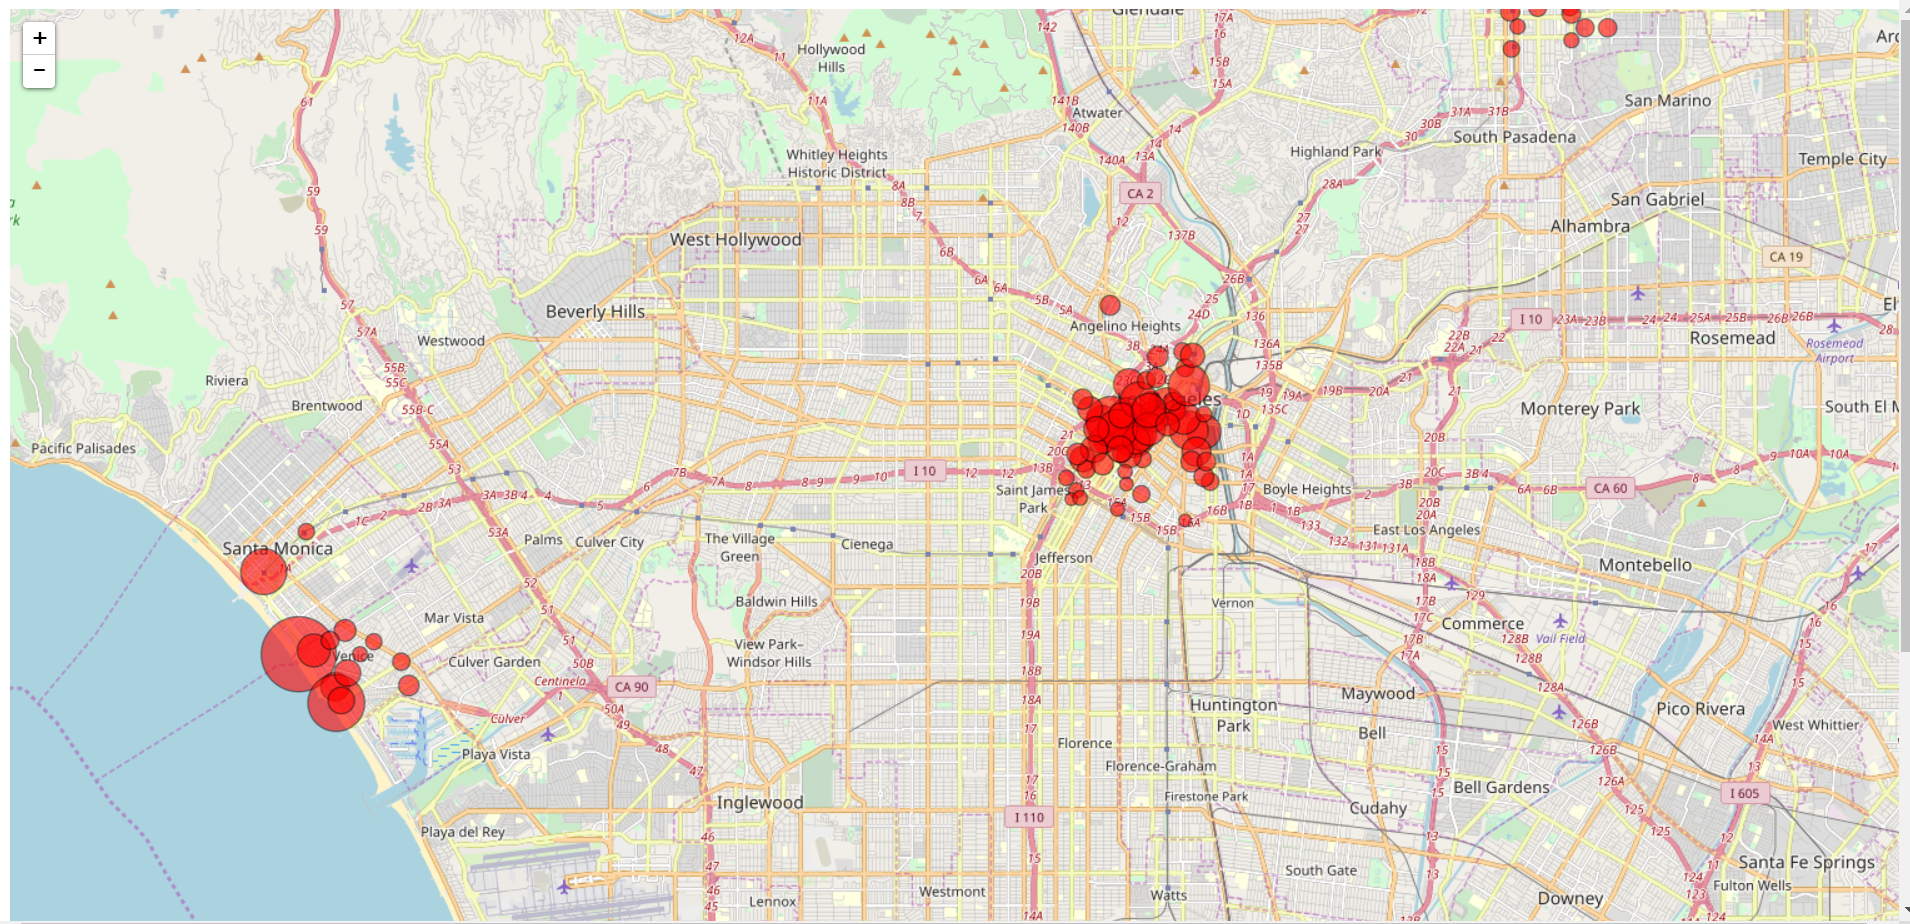
\includegraphics[scale=0.20]{figs/highlevel.PNG}
	\caption{\footnotesize{A high-level overview of current visualization}}
	\label{fig:First viz Chart}
	\captionsetup{justification=centering,margin=1cm}
	\vspace{-10pt}
\end{figure}
\subsubsection{Data Plotting}
After plotting the map of Los Angeles, we started with plotting the data points over this map. For the first visualization, we plotted the starting locations of all bike rides over the map. These were distinct locations in the map, defined by a latitude and longitude value. We used the data for the 1st quarter of 2018 as our seed data. The number of data points were in the order of 60,000 for a single quarter. For now, this data is loaded locally but as we include more data points for different quarters and years, we are planning to shift the data loading through a web server. This will considerably decrease the load time of the visualization.\\
The data points for our visualization are represented as circles of varying area (radius). The data is encoded in such a way that the radius linearly increases with the frequency of bike pick-ups for a given location. We keep the opacity of the circles to a value less than 1 so as to make the map visualization easier to understand and navigate. These circles are stroked with a minimum thickness to make them stand out when viewing from a zoomed-out perspective.
\begin{figure}[h]
	\centering % avoid the use of \begin{center}...\end{center} and use \centering instead (more compact)
	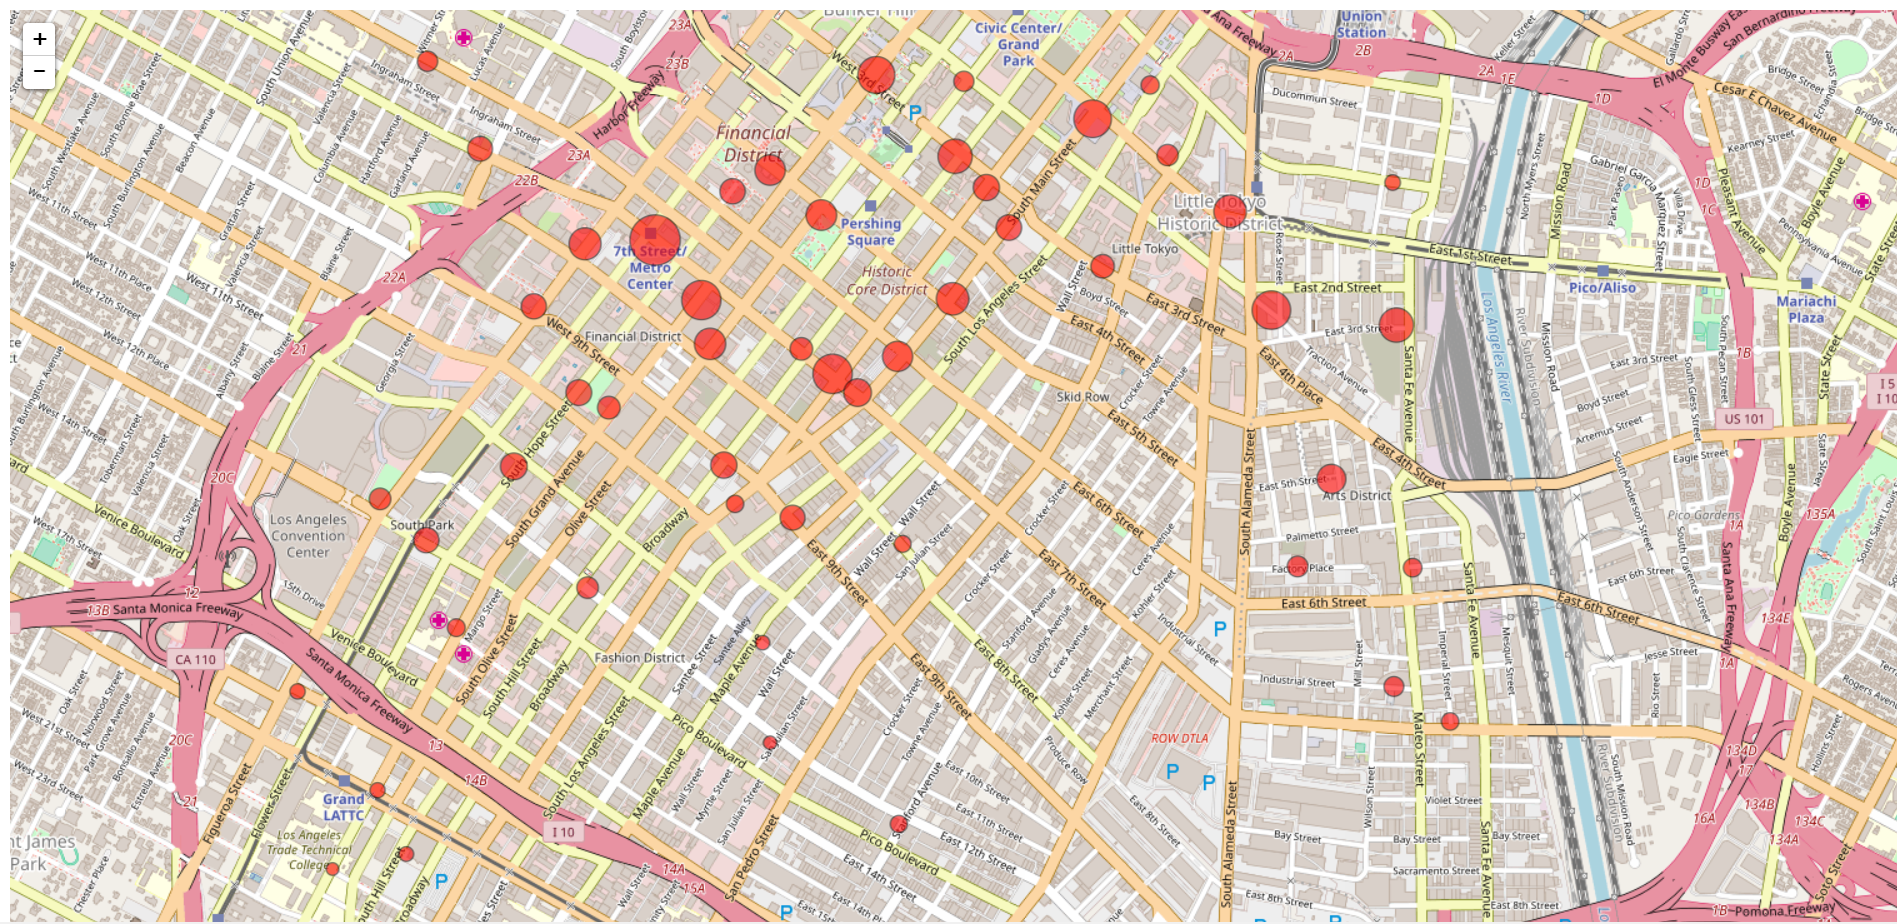
\includegraphics[scale=0.20]{figs/zoomedin.PNG}
	\caption{\footnotesize{A zoomed in view showing distinct geographic points}}
	\label{fig:First viz Chart}
	\captionsetup{justification=centering,margin=1cm}
	\vspace{-10pt}
\end{figure}
\subsection{User Interaction}
Our visualization design currently supports a number of interactions. These visualizations have been presented in the short movie as well. As work progresses on the visualization, these interactions will be enhanced and others added. For now, the following interactions are available to the user:
\begin{itemize}
    \item \textbf{Panning and Zooming}: The geographic map can be panned sideways to move around and locate different data points around the city. Also, the map can be zoomed in and out. Zooming in allows users to get a closer look into the data points on a street level view. This way the bike stations look more distinguishable from one another. The zoom feature here is constrained and semantic in nature. This interaction follows the Shneiderman's mantra of having an overview first and then allowing to zoom in and filter data.
    \item \textbf{Pop-up Effect}: The individual data points support a "On Click" feature. Every time a data point i.e. a circle is clicked, the color of the circle changes to blue with a more defined stroke around the circle. This makes the data point more visible and allows it to stand out, especially when there are a large number of similar data points around it. We decided on choosing the "On Click" action to show the effect rather than the "Hover" action since clicking an element to have a detailed overview of a single data point is more effective than hovering over it. Either ways, this follows the Shneiderman's Detail-on-Demand task taxonomy.
    \item \textbf{Tooltip}: In addition to the "On Click" feature changing the color of the circle, a tooltip will also appear on top of each data point. Currently, this tooltip shows the number of bike pick ups for a given location but a future enhancement might be to add a small visualization pertaining to the data within that geographic point.
\end{itemize}
\begin{figure}[h]
	\centering % avoid the use of \begin{center}...\end{center} and use \centering instead (more compact)
	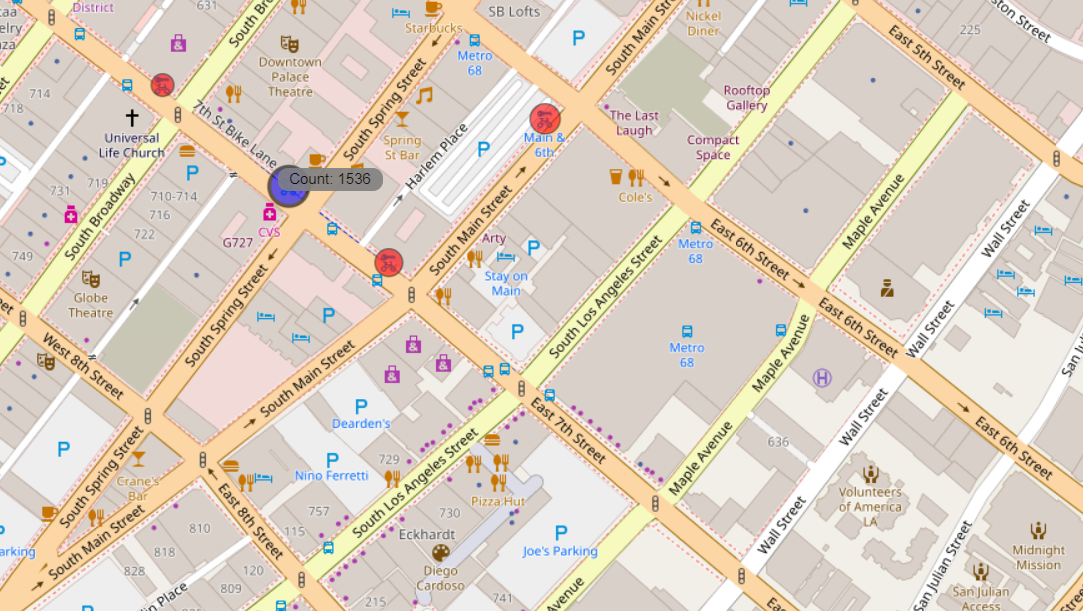
\includegraphics[scale=0.36]{figs/tooltip.png}
	\caption{\footnotesize{A simple tooltip implementation}}
	\label{fig:First viz Chart}
	\captionsetup{justification=centering,margin=1cm}
	\vspace{-10pt}
\end{figure}
This visualization has been coded by dividing the structure of the program into 3 segments:
\begin{itemize}
    \item PM3.html
    \item PM3.js
    \item PM3.css
\end{itemize}
As work progresses on the visualization, we plan on adding a histogram time frame at the bottom of the visualization window. This histogram will stretch the width of the window and allow users to cross-filter data in the map based on the selection in the histogram window.

\section{Evaluation} 
\label{sec:evaluation}

Our project can be put under the category of an application based visualization project. We used open-source data to create visualizations that help users identify trends and patterns in the way bike-share systems are being used in the city of Los Angeles. Keeping this in mind, we had planned our evaluation process to be primarily aimed at user test surveys.
The volunteers for user surveys can be one among the following:
\begin{enumerate}
	\item Mechanical Turks
	\item A group of people who can be considered as laymen in the field of data visualization
	\item A group of people with a considerable amount of idea and experience in the field of visualization design.
\end{enumerate}

Our evaluation approach included the last two groups of people from the list above. We decided not to move forward with performing evaluations on mechanical turks because we felt that for a project of our scale, being moderately complex and not too detailed, using the last two groups of people would suffice to come to a strong evaluation result. We explain each form of evaluation through the following sub-sections.

\subsection{Survey Users Q\&A}

This evaluation was based on asking our test users a number of questions with varying level of depth and accessing their answers in a qualitative and quantitative measure.

\subsubsection{Design}
As mentioned above, the user Q\&A session was primarily based on providing our test users with our visualization, making them study it in detail and then following it up with a number of questions. First off, we had to select the test users for our survey. Since this Q\&A session was aimed for laymen in the field of visualization, we selected friends who were not well acquainted with this subject matter as our test surveys. Our choice for only selecting laymen users was because the class presentation peer review would consist of review from a group of experienced data visualization users. To balance the selection, each project member initially selected two test subjects adding upto a total of six surveyors. Later, each member performed the evaluation on two more subjects each. This takes the total number of surveyors to 12.\newline
Then, we decided on method our survey. Each user was assigned to view and navigate through our visualization for 2 minutes. After this duration, the visualization was removed and they were handed a paper with a list of questionnaires. We wanted to see if our visualization design also had a sense of remembrance to it and by making the users answer questions by first removing the visualization we were able to test that to some extent. The questions were primarily of two kinds: open-ended and close-ended.\newline
The open-ended question pertained to the volunteers answering what they inferred from the overall visualization. This gave us a high-level feedback as to whether our choice of visualization fulfilled its initial objective. The close-ended questions will be more detailed and looked into whether the users were able to derive data and trends from the visualization. The rationale behind selecting these questions was to evaluate our design from both a high-level scenario and a detailed pattern finding scenario, which is ultimately the goal of the design. Some of the questions asked for each kind of questionnaire is listed below. A complete list of all the questions can be found in the \textbf{Evaluation} directory.
\begin{enumerate}
	\item Open-Ended Questions
	\begin{itemize}
		\item What can you infer from the visualization at a first glance?
		\item What do you think this visualization is trying to achieve?
		\item Does the visualization look appealing to you when you first see it?
	\end{itemize}
	\item Close-Ended Questions
	\begin{itemize}
		\item Which area of LA has more bike stations?
		\item How are the bike rents distributed across a certain area of bike stations?
		\item What overall trend can be inferred from the bike rent data?
	\end{itemize}
\end{enumerate}
We opted for comprehensive questions instead of multiple-answer questions which could ask subjects to answer from a list of 5 options ranging from 'Strongly Agree' to 'Strongly Disagree'. We decided on this because in addition to receiving positive/negative feedback, we also wanted feedback that would help us improve our design and add to it for future work. A simple multiple choice question would only provide us with a discrete result set for generalization.\newline
Each user was given 5 minutes to finish the questionnaire after which the answers were collected and analyzed. The answers from all test subjects were tallied and categorized broadly into two bins: positive and negative. The details from the answers were noted down which served well for our lessons learned and future work sections.
\subsubsection{Results}
The overall results from the user Q\&A session was positive. This section will talk about the summary of the observations and the responses received for the visualization design.\newline
Almost all the open-ended questions received positive responses. It could be concluded that the high-level goal was met by our visualization design. Out of the 12 participants, 10 answered positively on questions like "\textit{What do you think this visualization is trying to achieve?}". This gives us a success rate of 83.3\%. However, the reactions were a bit mixed towards the initial appeal of the visualization. Only 7 out of the 12 subjects positively responded towards the initial appeal and design. This makes up for 58.3\% of the subject population.\newline
Some comments about the design were directed towards the layout and look of the time histogram. We received feedback to make it more visually appealing and 6 of the subjects mentioned that the prevailing bug on our design was a a negative factor while the remaining half believed it did not act as a hindrance to their analysis.\newline
As for the close-ended questions, they were answered with relative ease. Tasks such as finding busiest bike stations and station distribution was done quickly and almost all the test subjects were able to determine the trend of bike rents. 11 out of the 12 subjects were successful in finding the trend of bike rents through time which is an accuracy of 91.6\%. We also tested the idea of remembrance to check how much of the visualization they still remember and received positive results as 9 out of 12 subjects agreed to remembering evey detail of the visualization (75\%).\newline
As mentioned before, all the answers of the questionnaire can be viewed in the \textbf{Evaluation} directory.
\subsection{Visualization Comparison}

This evaluation method is closely linked with the first method because it was performed at the same time one after the other. 
\subsubsection{Design}
In addition to finding out how our visualization design fared on its own (in terms of fulfilling its primary objectives), we also wanted to see how it compared to other visualizations that performed similar tasks as our design. Comparing two things which perform similar if not the same tasks is always a good way to check for effectiveness and efficiency. This test would expand our evaluation coverage in such a way that we could get more ideas and feedback about possible changes/addition to our design.\newline
Following from the first evaluation technique, we presented the test subjects with another visualization design. We chose the \textbf{Bike Visualization} website which contains the visualization of bike shares for a large number of locations. This design implements more interactions than our visualization and is much more complex than our system. So for the sake of equality in comparison, we decided to test this for the same tasks as that were performed on our visualization. We chose the \textbf{New York Citibike Visualization} where we asked our test users the same questions as before after letting them view and interact with the visualization for 2 minutes. In this case, we focused more on the close-ended questions since we wanted to compare trend finding and location finding tasks between the two visualizations.
\subsubsection{Results}
The results from the visualization comparison came out somewhat expected. The New York Citibike visualization had more features and interactions, making it more favored than our visualization. 11 out of the 12 test subjects leaned towards this visualization apporach (91.67\%).\newline
The open-ended questions provided similar results as well, both in terms of answer type and time to answer. These visualizations were built by a team of experts who had experience in the field of data visualization and hence the design choices made by them was sound and just. That makes the visualization look appealing and obtains the overall objective as well. All 12 out of 12 people liked the initial appeal of the visualization producing a success rate of 100\%. The same accuracy was obtained for questions like "\textit{What do you think this visualization is trying to achieve?}".\newline
Similarly, the close-ended questions did not vary as much from the answers of our visualization. The only noticeable difference was in the speed of answering. The test subjects seemed to take less time to find trends and locate items/places in the map compared to our visualization. This could be because of faster data processing and a smoother filtration process by the New York CitiBike visualization compared to our design.\newline
Overall, the visualization comparison resulted in test subjects favoring the New York CitiBike visualization over our visualization design.
\subsection{Class Peer Review}
This is the part of the evaluation where our visualization was reviewed by a group of students experienced in the field of data visualization.
\subsubsection{Design}
As part of our class project, we presented our visualization design to the class of CSC 544 - Advanced Data Visualization. There were 5 students and Professor Katherine Isaacs attending our presentation. During the presentation, we talked about the overview of our project, explained the methodology ranging from task and data abstraction to the design rationale. We explained our visualization design to the class along with a small demo. After the presentation, there was a round of Q\&A session where the students asked us a number of questions related to the project and also provided feedback. The students were then assigned to anonymously fill up a questionnaire designed by the Professor. The questionnaire was in the form of a Google Form and contained the following questions:
\begin{enumerate}
	\item What is the goal of this project? What problem is it trying to solve and why is that problem important?
	\item What are the strengths of the solution?
	\item What in the solution could be improved and how? (Do not repeat what the presenter has already said.)
\end{enumerate}
The answers from the questionnaire were then used to form our evaluation result.
\subsection{Results}
The answers to the questionnaires were analyzed and the following conclusions were drawn for each question:
\begin{enumerate}
	\item For the first question, all of the five reviewers accurately described the goal of the project including the problem its trying to solve and the importance of it. The responses matched our project goal to visualize the LA bike share system. For the importance of the problem, the responses varied from helping users see bike share trends to planning the distribution of bike shares from a commercial standpoint. All these responses do fall in the scope of importance of the problem.
	\item Our visualization received a number of positive reviews in terms of strengths. What was interesting was how varied the responses were between the five reviewers. This goes to show the advantage of using visualization experts for evaluation. Below are some of the strengths of the visualization as mentioned in the reviews:
	\begin{itemize}
		\item Good data source with large possibility for future design additions
		\item Smooth interactions in the visualization
		\item Trends were displayed in a pronounced and pre-attentive manner
		\item Low learning curve giving an intuitive sense to the visualization
		\item Detailed data and task abstraction
		\item Good and in-depth design rationale
		\item Detailed evaluation plan, especially the visualization comparison section
	\end{itemize}
	These reviews supported the positive feedback received from the previous two methods of evaluation.
	\item Along with the strengths, there were a number of areas of improvements that were mentioned. These points were noted on the reviews but were also discussed in the Q\&A session after the presentation. Some of the future areas of improvements are listed below:
	\begin{itemize}
		\item When zoomed out, the circles get large and end up overlapping and crowding each other. A better representation, maybe a voronoi diagram would be useful.
		\item The opacity of the circles are not low enough to not occlude the background so decreasing the opacity might be helpful in that.
		\item Adding a title to the visualization and labels to the graphs would be helpful.
		\item Adding a 'Play Button' animation that automatically cycles through each month of the time period to show the visualization would be a good design addition.
		\item Showing the destination when the source is clicked.
		\item Adding a button to reset the view of the map and center is back to the original location would be helpful in viewers to start over.
		\item Since this is a large project with good data source, using more attributes such as destination and trip route information to show more trends would add to the current progress.
		\item Showing the information of all the months at once using various color/color scales for each month might help in comparing the data between months.
		\item Being able to handle data with a longer time frame than the current two year frame.
	\end{itemize}
	The above ideas and recommendations for future improvements of the project matched with some of the future plans that we had as well.
\end{enumerate}
\subsection{Discussion}
Here, we talk about the results from our evaluations and how it shapes our current visualization and any future direction of it. In a nutshell, our visualization project was conceived in a very positive manner in terms of the problem it was trying to solve and the method implemented to solve it but it fell behind in terms of features and designs compared to other visualizations that perform the same task.\newline
Starting with the strengths, the results of the evaluation resulted showed that both the general audience as well as the experienced reviewers liked the implementation of the visualization design. The use of circles of varying radius to show different bike stations over the map of a city was a good design choice and the rationale behind the color/opacity of the marks was also received well. Most of the test subjects being able to answer both the open-ended high level questions and well as the close-ended trend finding questions added to the conclusion that the chosen design rationale suited well for the task performed. In addition to the design, our data/task abstraction and evaluation approach was also well received by the peer reviewers which in a resulted in our design choices being well-defined.\newline
Coming to the improvements, our visualization seemed to have large room for improvements and many possibilities for future work. This was evident from the visualization comparison and the peer reviews received from the presentation. The project idea we took on and the problem we tried to solve through it is of a large domain. Through the background research, we were aware of the variety of tasks and interactions that could be performed to solve this problem by using the raw data available to us. Our primary goal for this project was to design a visualization layout to solve the problem of finding the bike share trends and how it changed with respect to time. There are a number of areas where our design can be improved to better portray the information. Some of the more urgent improvements seem to be adding titles and labels to inform users about what is being visualized and modifying the way in which the data is mapped when zoomed out so that the circles don't crowd over each other.\newline
In addition to this, we have improvements of our own which were part of our milestone but could not be achieved in time. These include fixing some bugs related to data mapping and implementing a brush over the time histogram in order to select multiple months at a time. The results from the visualization comparison show that our data handling and processing could be improved to speed up the visualization and interactions. One way of doing this would be to load the data to a server and read through it instead of reading the data locally. This would also provide options for scalability which is another area of improvement. The New York CitiBike visualization shows us that there a number of attributes that can be mapped into the visualization to show more trends and make the analysis process more richer. Other improvements include making the interaction smoother and more user-friendly by adding automatic animations and map view reset buttons. These are great ideas that can be added to our visualization to improve user experience.\newline
In summary, the results from the evaluations show that our visualization project performs its intended task with high accuracy but at the same time needs improvements on its designs along with integration of other attributes to expand the data and trend analysis of the bike share system.
\subsection{Limitations}
While our evaluation approach produced acceptable results that concurred with the results from the peer review, there were a few limitations to our approach. First, the questions asked to the test subjects were of a kind that did not produce detailed answers. The questions were more focused upon whether someone understood the problem and the task being performed in the visualization and if a user could easily perform said task. While these questions are important in order to properly evaluate the effectiveness of the visualization design, questions similar to the ones asked in the peer review section would have helped us gain insights about what could be improved from a layman's perspective. Even though design suggestions from a visualization expert will always be more detailed, taking suggestions from these test subjects would have been beneficial. This is because they form a part of the demographic population who despite mostly being laymen in the field of visualization will be the largest proportion of consumers of this visualization. Even if their suggestions might be in the simple scope of improvements, they will directly be targeted towards improving the user experience. So, questions that ask the users about possible improvements and suggestions on the design will help in better directing the future efforts of the project.\newline
Another limitation was the ineffective implementation of quantitative evaluation. During our initial evaluation phase, we intended to time the users while they were answering the trend finding and data localization questions. Our aim was to compare the time taken by each user and get a general sense of the time it takes for them to solve these tasks. Then we had planned on timing them for the same tasks on the New York CitiBike visualization and comparing these two sets of data. Our method of having the test subjects first go through the visualization and then answer the questiona separately posed a problem in terms of timing them. This is because the amount of time spent by the users on answering the questions now also relied on how well they remembered the visualization itself. We wanted the time to be independent of this factor and only depend on how effective the visualization itself is. Though the first few evaluations were timed, we later discarded this approach and relied on a general sense of how long people took to answer the questions.\newline
One way of adding quantitative evaluation to our appoach would be to having the users solve some task or find some data while they are navigating the visualization. This way the timing data obtained would be a factor of the effectiveness of the visualization design alone. We think this would result in more accurate data and hence a better evaluation result.

\section{Lessons Learned} 
\label{sec:lessons_learned}

In the duration of developing this visualization and analyzing the data for visualization we have learned few noticeable things as follows:

\subsection{What lessons we learned that could possibly be transferred to other visualization problems and contexts?}

\begin{itemize}
\item The most important lesson we have learned in designing our visualization is to decide how the visualization shouldn't look and how visualization should look. We have had many brain storming discussions in this area with the team members.
\item A user-centered design approach can result in an intuitive interface, which, in turn, can open up new possibilities. In our visualization, the appropriate user interface can open new possibilities by providing a big picture of operation and information within the metro bike share system.
\item Our visualization provides a customized display of information. It shows the graphical representations of bike renting trends in Los Angleles area. They also can measure efficiencies and inefficiencies, quickly identify correlations, and illustrate trends. All of these features combine to help in making better-informed decisions about the sustainablity of the bike sharing system.
\item One challenge for our visualization is that the interpretation of data can be difficult. Another issue is that the greater transparency provided may not always be desirable. There is also a danger of accidentally filtering by the wrong information. 
\item The most important practice to follow when designing a visualization is to find out who the information consumers are and whether they are managing data, consuming reports, or both. 
\item We have to design the visualization around what the users need at their fingertips to analyze the data. To this end, get the requirements from users. Research what they need and want to see. Find out which searches they run the most often and which ones they should be running to analyze the trends in the data.
\item Use a whiteboard layout and requirements to develop standard visualization. Whenever possible, have the interactive parts perform more than one function, and allow interactive parts to be clickable for more information. Clicking a bar in the histogram, for example, could display more current bike renting numbers. When deciding on the appropriate interactions, be careful to select the interaction type that best conveys the information being displayed. 
\item The data can be complex. Mistakes like graphically representing non-quantitative data, can lead to confusing results. Other common mistakes include mixing and matching unrelated data and starting the visualization with a blank screen instead of showing important and relevant information. We need to show information that is usable to the viewer in some manner.
\item A thorough requirements analysis is part of designing a visualization. The design process is to build, evaluate, test, and refine prototypes.
\item Data may be missing, incomplete, inaccurate, incorrectly entered, inconsistently coded, diversely coded, duplicated, or use different standards. We need to cleanse the data properly before we start the visualization.
\item  The underlying technology can be important. If you have a system that uses a graphic that uses Flash, be aware that it won’t run on the iPad. You’ve got to keep in mind, that over time, the visualization needs to change or evolve to run on many different technologies.
\item Focus on identifying and understanding the problem you’ll be solving. You’ll never be able to solve every problem and overcome every data use barrier in one project. Work with your users to develop a specific focus and thoroughly understand the barriers and challenges from their perspectives so you can tackle the most pressing issues.
\item Engage the right people, as we need a diverse range of perspectives and experiences to uncover problems and co-create solutions. 

\end{itemize}



\section{Project Summary} 
\label{sec:project_summary}

 

\subsection{Project Summarization}
 
Bike sharing systems are gaining immense popularity as an alternative or complementary mode of urban transport. Bike sharing can provide an alternative to traditional modes of transport or, more likely a complementary service for solving the ”last mile problem” of getting from a public transportation stop to the final destination. The whole project is aimed at shedding light on how well the bike sharing model is working in the LA metropolitan area.  

\subsection{What we did during the course of the project?}

We worked with the data provided by Kaggle and the open source data from Metro Bike Share. The initial structure of the data was in CSV format, from which after primary data cleaning in python, we converted it to GeoJson format. We divided our tasks according to according to Shneiderman Task taxonomy which also conforms to our project goal. Then we proceeded to make the visualization. Our work was to create a geographic map detailing every station according to their longitude and latitude; along with the numbers of rentals from each of those stations. We also added a histogram for every month from July of 2016 to September of 2018, which we used for the selection of the rentals in that particular timeframe. 


\subsection{What contributions are presented in this milestone?}
 
In this milestone, our major focus was towards the evaluation of our visualization. So, for this purpose, we presented our visualization to a group of six people with some open-ended and close-ended questions. We also made a comparison of our visualization with another visualization with a somewhat equivalent goal. And in the end, we made a presentation in front of our class which was entirely comprised of people from visualization background and collected feedback.

\subsection{What contributions were presented in the previous milestones?}

In the previous milestone, our work was focus towards the collection of the data and making the visualization design. Milestone 1 was about the proposal of the project; in milestone 2 we worked on data and task abstraction and how to proceed with the preliminary design. In next milestone, we created our initial skeleton of the geographical map and in milestone 4 we finetuned the map, along with the tooltips and created the histogram for data filtering.




%\bibliographystyle{abbrv}
\bibliographystyle{abbrv-doi-hyperref}
%%use following if all content of bibtex file should be shown
\nocite{*}
\bibliography{PM5}
\end{document}

